\chapter{Discussion}
Please tell more about conclusion and how to the next work of this study.

\section{Imron Sumadireja / 1164076}
\subsection{Teori}
\begin{enumerate}

\item Jelaskan kenapa file suara harus di lakukan MFCC. Dilengkapi dengan ilustrasi atau gambar. \par
MFCC merupakan koefisien yang merepresentasikan audio. Ekstraksi ciri dalam proses ini ditandai dengan pengubahan data suara menjadi citra berupa spektrum gelombang. File audio dilakukan MFCC itu agar objek suara dapat diubah menjadi bentuk matrix. Suara tersebut akan menjadi vektor yang nantinya akan diolah sebagai keluaran. Untuk ilustrasi sederhananya bisa dilihat pada gambar \ref{cc1}. Gambar tersebut menjelaskan tahapan-tahapan kenapa file suara harus dilakukan MFCC. Selain itu untuk memberikan kemudahan kepada mesin dalam mempelajari suara tersebut karena mesin tidak dapat membaca teks maka dari itu diperlukan MFCC untuk merubah suara tersebut menjadi vektor.
		\begin{figure}[!htbp]
		\centerline{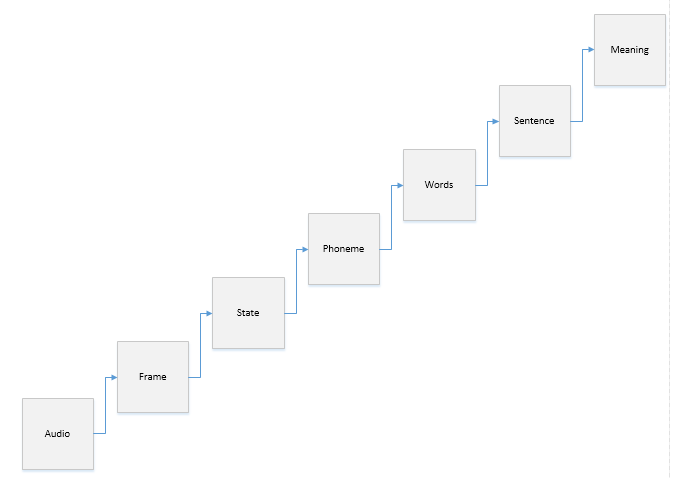
\includegraphics[width=0.5\textwidth]{figures/im/cc1.png}}
		\caption{MFCC.}
		\label{cc1}
		\end{figure}

\item Jelaskan konsep dasar neural network. Dilengkapi dengan ilustrasi atau gambar. \par
Konsep sederhana dari neural network hampir mirip dengan proses belajar pada anak-anak yakni dengan memetakan pola baru yang didapatkan dari inputan untuk membuat pola baru pada keluaran. Contoh sederhana tersebut menganalogikan kinerja otak manusia. Neural network itu sendiri terdiri dari sebuah unit pemroses yang disebut neuron yang berisi adder dan fungsi aktivasi. Fungsi aktivasi itu sendiri untuk mengatur keluaran yang diberikan oleh neuron. Neural network ini mengadopsi mekanisme berpikir sebuah sistem atau aplikasi yang menyerupai otak manusia, baik untuk pemrosesan berbagai sinyal elemen yang diterima, toleransi terhadap kesalahan/error, dan juga prallel processing. Karakteristik dari neural network dilihat dari pola hubungan antar neuron, metode penentuan bobot dari tiap koneksi, dan fungsi aktivasinya. Untuk ilustrasinya bisa dilihat pada gambar \ref{cc2}
		\begin{figure}[!htbp]
		\centerline{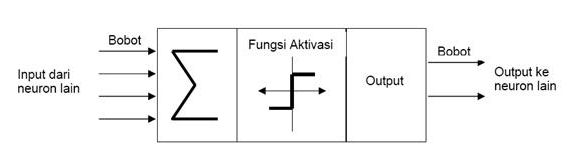
\includegraphics[width=0.5\textwidth]{figures/im/cc2.png}}
		\caption{Konsep Dasar Neural Network.}
		\label{cc2}
		\end{figure}

\item Jelaskan konsep pembobotan dalam neural network. Dilengkapi dengan ilustrasi atau gambar. \par
Pembobotan ini akan menentukan serta penanda dari sebuah konektivitas. Pada proses neural network dimulai dari input yang diterima oleh neuron beserta dengan nilai bobot dari tiap-tiap input yang ada. Setelah masuk ke dalam neuron, nilai input yang ada akan dijumlahkan oleh suatu fungsi penambahan. Hasil penjumlahan tersebut akan diproses oleh fungsi aktivasi oleh setiap neuron, hasil penjumlahan tersebut akan dibandingkan dengan nilai ambang tertentu. Jika nilai dari hasil penjumlahan tersebut melebihi nilai ambang maka aktivasi neuron akan dibatalkan, namun sebaliknya jika hasil penjumlahan dibawah nilai ambang maka neuron akan diaktifkan. Setelah neuron aktif selanjutnya akan mengirimkan nilai output melalui bobot-bobot keluarannya ke semua neuroon yang berhubungan. Ilustrasinya bisa dilihat pada gambar \ref{cc3}
		\begin{figure}[!htbp]
		\centerline{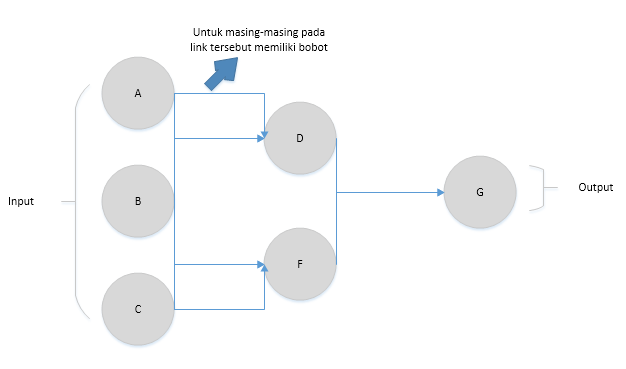
\includegraphics[width=0.5\textwidth]{figures/im/cc3.png}}
		\caption{Konsep Pembobotan Neural Network.}
		\label{cc3}
		\end{figure}

\item Jelaskan konsep fungsi aktifasi dalam neural network. Dilengkapi dengan ilustrasi atau gambar. \par
Fungsi aktivasi ini merupakan operasi matematik yang dikenakan pada sinyal output. Fungsi ini digunakan untuk mengaktifkan atau menonaktifkan neuron. Fungsi aktivasi ini terbagi setidaknya menjadi 6, dianranya sebagai berikut:
\begin{itemize}
\item a. Fungsi Undak Biner Hard Limit, fungsi ini biasanya digunakan oleh jaringan lapiran tunggal untuk mengkonversi nilai input dari suatu variabel yang bernilai kontinu ke suatu nilai output biner 0 atau 1.
\item b. Fungsi Undak Biner Threshold, fungsi ini menggunakan nilai ambang sebagai batasnya.
\item c. Fungsi Bipolar Symetric Hard Limit, fungsi ini memiliki output bernilai 1, 0 atau -1.
\item d. Fungsi Bipolar dengan Threshold, fungsi ini mempunyai output yang bernilai 1, 0 atau -1 untuk batas nilai ambang tertentu.
\item e. Fungsi Linear atau Identitas.
\end{itemize}
Untuk ilustrasi sederhananya bisa dilihat pada gambar \ref{cc4}. Gambar tersebut merupakan salah satu contoh dari fungsi aktivasi bipolar.
		\begin{figure}[!htbp]
		\centerline{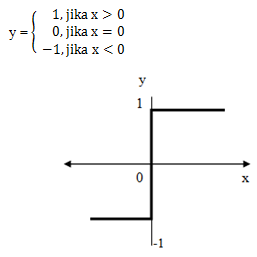
\includegraphics[width=0.5\textwidth]{figures/im/cc4.png}}
		\caption{Konsep Fungsi Aktivasi Neural Network.}
		\label{cc4}
		\end{figure}

\item Jelaskan cara membaca hasil plot dari MFCC. Dilengkapi dengan ilustrasi atau gambar. \par
Membaca plot MFCC ini bisa kita lihat pada gambar \ref{cc5}. Gambar tersebut menjelaskan bahwa pada waktu ke 5 daya atau desible yang dikelurakan pada nada tersebut paling keras pada 20 Hz, selain itu pada 40 -120 Hz itu daya atau desible yang dikeluarkan pada musik yang telah di plotting. Begitupun seterusnya bahwa warna yang paling gelap itu merupakan daya atau desible yang paling tinggi dibandingkan dengan warna yang cerah. Untuk yang berwarna merah itu suara dibawah pendengaran frekuensi manusia, jadi tidak dapat terdengar secara langsung. 
		\begin{figure}[!htbp]
		\centerline{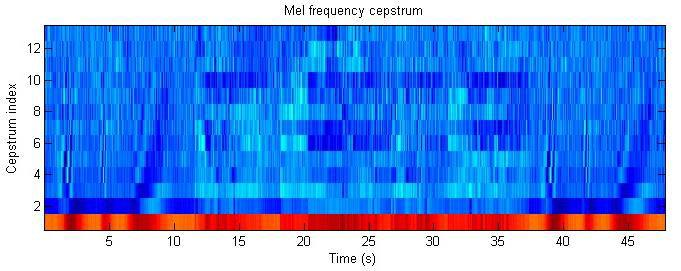
\includegraphics[width=0.5\textwidth]{figures/im/cc5.png}}
		\caption{Membaca Plot MFCC.}
		\label{cc5}
		\end{figure}

\item Jelaskan apa itu one-hot encoding. Dilengkapi dengan ilustrasi kode dan atau gambar. \par
Sederhananya one-hot encoding ini untuk merubah hasil data vektorisasi menjadi bilangan biner 0 dan 1 serta membuat keterangan pada atribut tersebut menjadi label. Unutuk ilustrasi sederhananya bisa dilihat pada gambar \ref{cc6}
		\begin{figure}[!htbp]
		\centerline{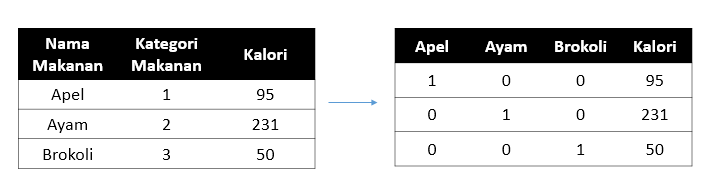
\includegraphics[width=0.5\textwidth]{figures/im/cc6.png}}
		\caption{One-Hot Encoding.}
		\label{cc6}
		\end{figure}

\item Jelaskan apa fungsi dari np.unique dan to categorical dalam kode program. Dilengkapi dengan ilustrasi atau gambar. \par
Fungsi dari np.unique adalah untuk menemukan elemen yang berbeda atau unik array, dan dapat mengembalikan elemen unik array tersebut yang diurutkan. Untuk ilustrasi sederhananya bisa dilihat pada gambar \ref{cc7}. Gambar tersebut menjelaskan bahwa unique itu sendiri akan mengambil data yang berbeda dari variabel a yang berada dalam fungsi array dan hasilnya seperti gambar tersebut.
		\begin{figure}[!htbp]
		\centerline{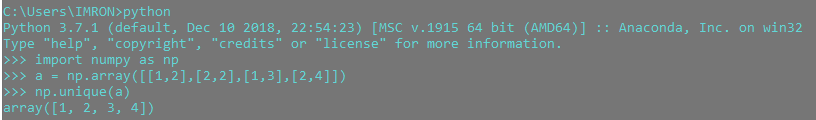
\includegraphics[width=0.5\textwidth]{figures/im/cc7.png}}
		\caption{np.unique.}
		\label{cc7}
		\end{figure}

Fungsi dari to\_categorical untuk mengubah vektor yang berupa integer menjadi matrix dengan kelas biner. Untuk ilustrasinya bisa dilihat pada gambar \ref{cc71}
		\begin{figure}[!htbp]
		\centerline{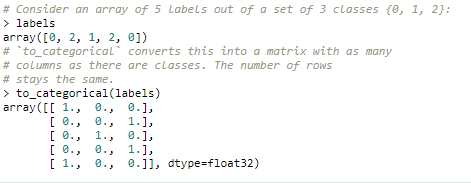
\includegraphics[width=0.5\textwidth]{figures/im/cc71.png}}
		\caption{to\_categorical.}
		\label{cc71}
		\end{figure}

\item Jelaskan apa fungsi dari Sequential dalam kode program. Dilengkapi dengan ilustrasi atau gambar.\par
Salah satu jenis model yang digunakan dalam perhitungan. Sequential ini membangun tumpukan linear yang berurutan. Contoh sederhananya sebagai berikut \ref{cc8}
		\begin{figure}[!htbp]
		\centerline{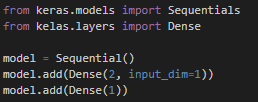
\includegraphics[width=0.5\textwidth]{figures/im/cc8.png}}
		\caption{Sequential.}
		\label{cc8}
		\end{figure}

\end{enumerate}

\section{Yusniar Nur Syarif Sidiq / 1164089}
\subsection{Pemahaman Teori Yusniar Nur Syarif Sidiq / 1164089}
\begin{enumerate}

\item Jelaskan kenapa file suara harus di lakukan MFCC. dilengkapi dengan ilustrasi !
	\subitem MFCC (Mel Frequency Cepstrum Coefficients) merupakan metode untuk melakukan feature extraction, sebuah proses yang mengkonversikan signal suara menjadi beberapa parameter. Dimana dalam python MFCC digunakan untuk melakukan etraction suara menjadi bentuk vektor. Mengapa perlu dilakukan ?, dikarenakan mesin tidak dapat membaca data selain bilangan biner dan vektor, maka dari itu untuk mempermudah pembacaan data oleh mesi perlu dilakukannya MFCC. Disini saya akan memberikan ilustrasi sederhana dimana ada sebuah Mechine Learning yang ingin membaca data dalam bentuk gelombang suara. Mechine Learning tidak akan bisa membaca data tersebut, Mengapa ?, karena data tersebut masih berbentuk gelombang suara, untuk memahami Mechine Learning perlu data dalam bentuk vektor, maka gelombang suara tersebut akan diubah menjadi bentuk vektor.

\item Jelaskan konsep dasar neural network. Dilengkapi dengan ilustrasi atau gambar !
	\subitem Neural Network atau Jaringan Saraf dimana memiliki neuron dan pada tiap neuron akan saling terhubung pada lapisan - laposan berikutnya. Pada lapisan pertama dimana terjadinya proses menerima input sedangkan pada lapisan terakhir akan memberikan output. Neural Network akan mengadopsi mekanisme berpikir sebuah sistem atau aplikasi yang menyerupai otak manusia, baik dalam pemrosesan berbagai sinyal elemen yang diterima, toleransi kesalahan atau error, dan parallel processing. Dimana terdapat dua data apel dan jeruk, data tersebut akan diinputkan pada setiap layer. Data tersebut akan dilakukan proses hidden pada hidden layer. Data yang dinputkan tadi akan diubah kedalam bentuk binner, dan outputnya akan terjadi misalnya 01 itu adalah apel dan 10 itu adalah jeruk. Untuk contoh figure dapat dilihat pada figure \ref{YNC6-1}.

	\begin{figure}[!htbp]
		\centering{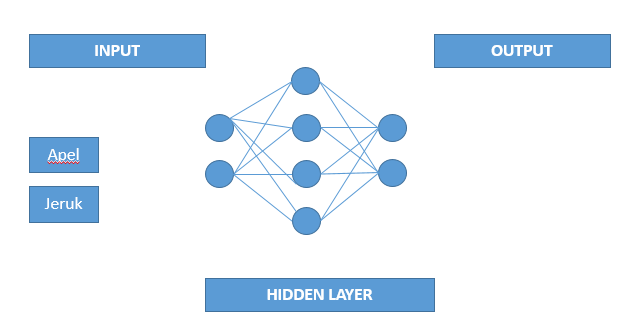
\includegraphics[scale=0.5]{figures/YN/Chapter6/Teori/YNC6-1.png}}
		\caption{Konsep Nural Network}
		\label{YNC6-1}
	\end{figure}

\item Jelaskan konsep pembobotan dalam neural network. Dilengkapi dengan ilustrasi atau gambar !
	\subitem Dimana Bobot akan mewakili koneksi antar unit. Apabila bobot dari node 1 ke node 2 memiliki nilai yang kebih besar, hal ini menandakan bahwa neuron 1 memiliki pengaruh yang lebih besar terhadap neuron 2. Apabila nilai bobot mendekati nol hal ini menandakan akan merubah input namun tidak mengubah output dan apabila nilai bobot negatif hal ini menandakan akan meningkatkan input namun mengurangi output yang artinya bobot akan menentukan seberapa besar pengaruh input terhadap output. Untuk ilustrasi figure dapat dilihat pada figure \ref{YNC6-2}.

	\begin{figure}[!htbp]
		\centering{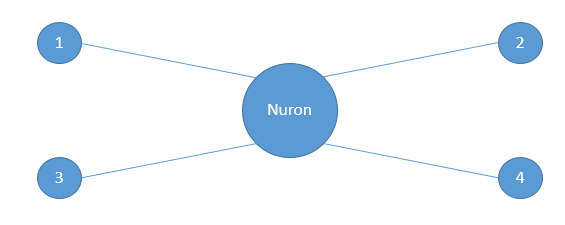
\includegraphics[scale=0.5]{figures/YN/Chapter6/Teori/YNC6-2.png}}
		\caption{Konsep Pembobotan}
		\label{YNC6-2}
	\end{figure}	

\item Jelaskan konsep fungsi aktivasi dalam neural network. Dilengkapi dengan ilustrasi atau gambar !
	\subitem Dimana fungsi aktivasi ini merupakan operasi dalam matematika yang digunakan pada sinyal output y. Fungsi ini sering digunakan untuk mengaktifkan atau menonaktifkan neuron. Dimana perilaku dari nural network ini ditentukan oleh bobot dan input-output fungsi aktivasi yang telah ditetapkan. Contohnya dimana jaringan lapisan tunggal akan menkonversi nilai input dari suatu variabel yang bernilai continue ke suatu nilai output biner yaitu angka 0 dan 1. Untuk contoh figure dapat dilihat pada pada figure \ref{YNC6-3}

	\begin{figure}[!htbp]
		\centering{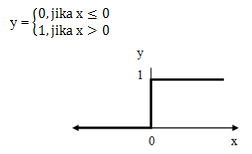
\includegraphics[scale=0.5]{figures/YN/Chapter6/Teori/YNC6-3.png}}
		\caption{Fungsi Aktivasi}
		\label{YNC6-3}
	\end{figure}	
	
\item Jelaskan cara membaca hasil plot dari MFCC. Dilengkapi dengan ilustrasi atau gambar !
	\subitem Perhatikan figure \ref{YNC6-4}, dimana terlihat bahwa warna biru merupakan suara terendah, mengapa ?, dikarenakan warna biru bernilai -300, sedangkan warna merah merupakah suara tertinggi dan bernilai 200. Jika diilustrasikan ada sebuah musik yang sedang dimainkan dan diperoleh datanya lalu diplot, maka akan terlihat seperti pada figure \ref{YNC6-4}

	\begin{figure}[!htbp]
		\centering{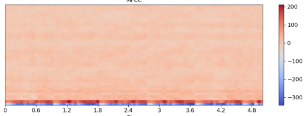
\includegraphics[scale=0.5]{figures/YN/Chapter6/Teori/YNC6-4.png}}
		\caption{Plot MFCC}
		\label{YNC6-4}
	\end{figure}	

\item Jelaskan apa itu one-hot encoding. Dilengkapi dengan ilustrasi kode dan atau gambar !
	\subitem One-hot encoding merupakan representasi variabel berkategorikan sebagai vektor biner yang artinya hanya akang 0 dan 1. Dimana mengharuskan nilai categorinya berbentuk biner dan setiap nilai integer akan dipresentasikan kedalam vektor biner. Contoh figure dapat dilihat pada figure \ref{YNC6-5}

	\begin{figure}[!htbp]
		\centering{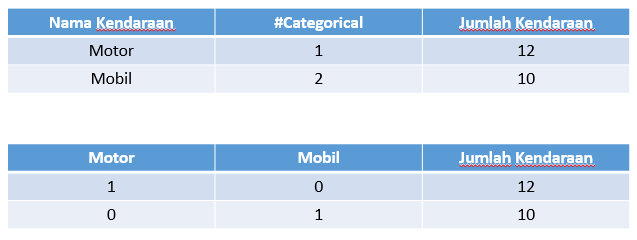
\includegraphics[scale=0.5]{figures/YN/Chapter6/Teori/YNC6-5.png}}
		\caption{One-Hot Encoding}
		\label{YNC6-5}
	\end{figure}	

\item Jelaskan apa fungsi dari np.unique dan to\_categorical dalam kode program . Dilengkapi dengan ilustrasi atau gambar !
	\subitem Fungsi dari np.unique yaitu sebagai indeks array input yang memberikan nilai unik, sebagai indeks array unik yang merekonstruksi array input, dan menghitung berapa kali setiap nilai unik muncul dalam array input. Contoh source code dalam pemrograman dapat dilihat pada figure \ref{YNC6-6}

	\begin{figure}[!htbp]
		\centering{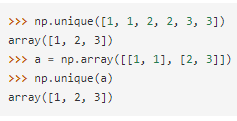
\includegraphics[scale=0.5]{figures/YN/Chapter6/Teori/YNC6-6.png}}
		\caption{np.unique}
		\label{YNC6-6}
	\end{figure}	

	\subitem Fungsi dari to\_categorical yaitu untuk mengubah vektor ke dalam matriks class biner. Contoh source code to\_categorical dapat dilihat pada figure \ref{YNC6-7}

	\begin{figure}[!htbp]
		\centering{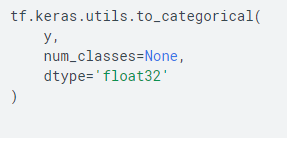
\includegraphics[scale=0.5]{figures/YN/Chapter6/Teori/YNC6-7.png}}
		\caption{categorical}
		\label{YNC6-7}
	\end{figure}	

\item Jelaskan apa fungsi dari Sequential dalam kode program. Dilengkapi dengan ilustrasi atau gambar !
	\subitem Dimana fungsi dari Sequential dalam source code program hanyalah sebagai tumpukan linear lapisan, dimana contih source code dalam program dapat dilihat pada figure \ref{YNC6-8}

	\begin{figure}[!htbp]
		\centering{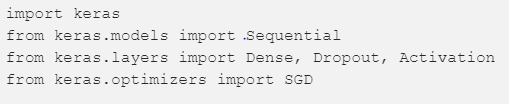
\includegraphics[scale=0.5]{figures/YN/Chapter6/Teori/YNC6-8.png}}
		\caption{Sequential}
		\label{YNC6-8}
	\end{figure}

\end{enumerate}